
\mychapter{Exploitation des données}
%----------------------------------
\section{Introduction}
%----------------------------------

Dans ce chapitre, nous présentons les deux composantes analytiques de notre système :
la Business Intelligence (BI) et l'Intelligence Artificielle (IA). La BI regroupe
l'ensemble des tableaux de bord interactifs et des indicateurs de performance permettant
le pilotage de l'activité commerciale en temps réel. L'IA, quant à elle, est mise en
œuvre à travers un module de prévision des ventes basé sur la régression linéaire,
visant à anticiper les tendances futures de l'activité.

%----------------------------------
\section{Business Intelligence}
%----------------------------------

Face à la concurrence croissante et à la complexité des marchés, les entreprises
ne peuvent plus se contenter de gérer leurs données a posteriori. L'analyse prédictive
est devenue un levier essentiel pour anticiper les tendances, identifier les risques
et optimiser la prise de décision.

\subsection{Définition}

La Business Intelligence (BI) est un processus technologique d'analyse des données
et de présentation d'informations pour aider à prendre des décisions sures,
Dans le cadre de notre système, la BI englobe l'ensemble des outils et méthodologies
mis en place des modules de ventes, clients, produits et facturation. Ces données
sont ensuite traitées et préparées pour l'analyse, afin de créer des tableaux de bord
interactifs, des indicateurs de performance (KPIs) et des graphiques de visualisation,
afin de prendre des décisions basées sur des données concrètes \cite{oracle_bi}.

%----------------------------------
\subsection{Application de la méthode GIMSI}
%----------------------------------

La structure de notre partie BI s'appuie sur la méthode GIMSI, dont nous avons
appliqué 7 étapes réparties sur 3 phases. Chacune de ces étapes a été traitée
dans les différents chapitres du présent rapport, comme détaillé dans le
tableau~\ref{tab:gimsi}.

\vspace{6pt}

\begin{longtable}{|>{\centering\arraybackslash}p{3cm}|>{\centering\arraybackslash}p{0.8cm}|>{\bfseries\raggedright\arraybackslash}p{3.5cm}|>{\raggedright\arraybackslash}p{5cm}|}
\hline
\rowcolor{blue!20}
\textcolor{black}{\textbf{Phase}} &
\textcolor{black}{\textbf{Étape}} &
\textcolor{black}{\textbf{Intitulé}} &
\textcolor{black}{\textbf{Description}} \\
\hline
\endfirsthead
\hline
\rowcolor{blue!20}
\textcolor{black}{\textbf{Phase}} &
\textcolor{black}{\textbf{Étape}} &
\textcolor{black}{\textbf{Intitulé}} &
\textcolor{black}{\textbf{Description}} \\
\hline
\endhead
\multirow{2}{3cm}{\centering\textbf{Phase 1}\\\textbf{Identification}} &
1 & Environnement de l'entreprise &
Analyse de l'environnement économique et de la stratégie afin de définir le périmètre
et la portée du projet (voir Chapitre~1). \\
\cline{2-4}
& 2 & Identification de l'entreprise &
Identification des structures, processus, activités et acteurs concernés
(voir Chapitres~1 et~2). \\
\hline
\multirow{3}{3cm}{\centering\textbf{Phase 2}\\\textbf{Conception}} &
3 & Définition des objectifs &
Définition des objectifs décisionnels en lien avec les besoins stratégiques
(voir Chapitre~2). \\
\cline{2-4}
& 4 & Construction du tableau de bord &
Conception des tableaux de bord adaptés aux besoins de chaque acteur
(voir Chapitre~3). \\
\cline{2-4}
& 5 & Choix des indicateurs &
Sélection des indicateurs clés de performance (KPIs) en fonction des objectifs
et du contexte de l'entreprise (voir Chapitre~4). \\
\cline{2-4}
& 7 & Système de tableaux de bord &
Construction et intégration du système complet de tableaux de bord interactifs
(voir Chapitre~4). \\
\hline
\textbf{Phase 3}\newline\textbf{Mise en œuvre} &
9 & Intégration et déploiement &
Déploiement de la solution complète au sein de l'environnement de l'entreprise
(voir Chapitre~5). \\
\hline
\caption{Application de la méthode GIMSI}
\label{tab:gimsi}
\end{longtable}

\subsection*{Conception des Indicateurs Clés de Performances}
\label{sec:ch3:kpi}
\addcontentsline{toc}{subsection}{Conception des Indicateurs Clés de Performances}

\vspace{6pt}

\begin{longtable}{|>{\centering\arraybackslash\bfseries}p{2.5cm}|>{\raggedright\arraybackslash}p{4cm}|>{\raggedright\arraybackslash}p{4cm}|>{\centering\arraybackslash}p{1.8cm}|>{\centering\arraybackslash}p{1.5cm}|}
\hline
\rowcolor{blue!20}
\textcolor{black}{\textbf{KPI}} &
\textcolor{black}{\textbf{Description}} &
\textcolor{black}{\textbf{Formule}} &
\textcolor{black}{\textbf{Graphique}} &
\textcolor{black}{\textbf{Couleur}} \\
\hline
\endfirsthead
\hline
\rowcolor{blue!20}
\textcolor{black}{\textbf{KPI}} &
\textcolor{black}{\textbf{Description}} &
\textcolor{black}{\textbf{Formule}} &
\textcolor{black}{\textbf{Graphique}} &
\textcolor{black}{\textbf{Couleur}} \\
\hline
\endhead
Chiffres d'affaires total &
Cet indicateur est chargé d'afficher le montant global de l'ensemble des ventes actives. &
CA total = Somme des ventes actives &
Carte avec icône &
\colorswatch{blue!70!black} \\
\hline
Chiffres d'affaires mensuel &
Cet indicateur est chargé d'afficher le montant des ventes effectuées dans le mois souhaité. &
CA mensuel = Somme des ventes du mois souhaité &
Carte avec icône &
\colorswatch{blue!50} \\
\hline
Panier Moyen &
Cet indicateur est chargé de mesurer le revenu moyen généré par chaque vente effectuée. &
Panier moyen = CA Total / Nombre de ventes &
Carte avec icône &
\colorswatch{violet} \\
\hline
\textcolor{blue!70!black}{Taux de Croissance} &
Cet indicateur est chargé de mesurer la variance du chiffre d'affaires par rapport au mois précédent. &
Croissance = [CA(n) - CA(n-1)] / CA(n-1) x 100 &
Carte avec icône &
\begin{tabular}[c]{@{}c@{}}
\colorswatch{green!60!black}\\[-2pt]
{\tiny Vert si positif}\\[4pt]
\colorswatch{red!70}\\[-2pt]
{\tiny Rouge si négatif}\\[4pt]
\colorswatch{gray!50}\\[-2pt]
{\tiny Gris si nul}
\end{tabular} \\
\hline
\textcolor{blue!70!black}{Taux de marge} &
Cet indicateur est chargé de mesurer le gain réalisé sur les ventes enregistrées, correspondant à la différence entre le chiffre d'affaires et le coût d'achat. &
Marge brute = quantité x (prix\_vente - prix\_achat)

\vspace{4pt}
Taux de marge = marge brute / (quantité x prix\_vente) x 100 &
Carte avec icône &
\colorswatch{orange!80!black} \\
\hline
\caption{Conception des Indicateurs Clés de Performances}
\label{tab:kpi-generaux}
\end{longtable}

\newpage

\subsection*{Conception des KPIs — Tableau de Bord Chiffre d'Affaires}
\addcontentsline{toc}{subsection}{Conception des KPIs — Tableau de Bord Chiffre d'Affaires}

\begin{longtable}{|>{\centering\arraybackslash\bfseries}p{2.5cm}|>{\raggedright\arraybackslash}p{3.5cm}|>{\raggedright\arraybackslash}p{4cm}|>{\centering\arraybackslash}p{1.8cm}|>{\centering\arraybackslash}p{1.5cm}|}
\hline
\rowcolor{blue!20}
\textcolor{black}{\textbf{KPI}} &
\textcolor{black}{\textbf{Description}} &
\textcolor{black}{\textbf{Formule}} &
\textcolor{black}{\textbf{Graphique}} &
\textcolor{black}{\textbf{Couleur}} \\
\hline
\endfirsthead
\hline
\rowcolor{blue!20}
\textcolor{black}{\textbf{KPI}} &
\textcolor{black}{\textbf{Description}} &
\textcolor{black}{\textbf{Formule}} &
\textcolor{black}{\textbf{Graphique}} &
\textcolor{black}{\textbf{Couleur}} \\
\hline
\endhead
Évolution du chiffre d'affaires &
Ce graphique est chargé d'afficher l'évolution du chiffre d'affaires et du volume de ventes enregistrés mois par mois ou semaine par semaine. &
Chiffres d'affaire = Somme de total (par mois/par semaine)

\vspace{4pt}
Nombres des ventes = Count nombre ventes (par mois/par semaine) &
Graphique combiné (Barres + Aires)

\vspace{4pt}
\textit{Info\_bulle} (affiche le CA et nombre de ventes) &
\begin{tabular}[c]{@{}c@{}}
\colorswatch{blue!70!black}\\[-2pt]
{\tiny Barres}\\[6pt]
\colorswatch{blue!30}\\[-2pt]
{\tiny Aire}
\end{tabular} \\
\hline
Anomalies CA &
Est chargé d'afficher les jours anormaux du chiffre d'affaires détectés sur la période. &
Moyenne = CA/jour / nombre-jour

\vspace{4pt}
Ecart\_type = racine( somme(CA\_jour - Moyenne)\textsuperscript{2} / n )

\vspace{4pt}
Z\_score = (CA/jour - moyenne) / ecart\_type &
Graphique en aires &
\begin{tabular}[c]{@{}c@{}}
\colorswatch{blue!30}\\[-2pt]
{\tiny Aire normale}\\[4pt]
\colorswatch{red!80}\\[-2pt]
{\tiny Pic anormal}\\[4pt]
\colorswatch{orange!80}\\[-2pt]
{\tiny Creux anormal}
\end{tabular} \\
\hline
Top 5 Produits par Chiffre d'affaires &
Cette section est chargée de classer et afficher les 5 produit ayant généré plus de chiffres d'affaires. &
CA Total d'affaire par produit = Somme de sous total (par produit)

\vspace{4pt}
Trié en ordre décroissant (5 premiers résultats) &
Liste classée &
\\
\hline
Répartition du CA Par produit/Catégorie &
Cette section est chargée d'afficher la contribution proportionnelle de chaque produit au chiffre d'affaires regroupé par catégories. &
Répartition du CA d'affaire par produit = CA par produit / CA total

\vspace{4pt}
Répartition du CA d'affaires par Catégories = CA par catégories / CA total &
Diagramme en secteurs

\vspace{4pt}
\textit{Info\_bulle} (affiche nom de produit + CA en TND)

\vspace{4pt}
\textit{Panneau de légende} (affiche nom de catégorie + CA + répartition) &
\begin{tabular}[c]{@{}c@{}}
\colorswatch{blue!70!black}\\[-2pt]
{\tiny Rang 1}\\[4pt]
\colorswatch{blue!55}\\[-2pt]
{\tiny Rang 2}\\[4pt]
\colorswatch{blue!40}\\[-2pt]
{\tiny Rang 3}\\[4pt]
\colorswatch{blue!25}\\[-2pt]
{\tiny Rang 4}\\[4pt]
\colorswatch{blue!10}\\[-2pt]
{\tiny Rang 5}
\end{tabular} \\
\hline
\caption{Conception des KPIs — Tableau de Bord Chiffre d'Affaires}
\label{tab:kpi-ca}
\end{longtable}

\newpage

\subsection*{Conception des KPIs — Tableau de Bord Clients}
\addcontentsline{toc}{subsection}{Conception des KPIs — Tableau de Bord Clients}

\begin{longtable}{|>{\centering\arraybackslash\bfseries}p{2.5cm}|>{\raggedright\arraybackslash}p{3.5cm}|>{\raggedright\arraybackslash}p{4cm}|>{\centering\arraybackslash}p{1.8cm}|>{\centering\arraybackslash}p{1.5cm}|}
\hline
\rowcolor{blue!20}
\textcolor{black}{\textbf{KPI}} &
\textcolor{black}{\textbf{Description}} &
\textcolor{black}{\textbf{Formule}} &
\textcolor{black}{\textbf{Graphique}} &
\textcolor{black}{\textbf{Couleur}} \\
\hline
\endfirsthead
\hline
\rowcolor{blue!20}
\textcolor{black}{\textbf{KPI}} &
\textcolor{black}{\textbf{Description}} &
\textcolor{black}{\textbf{Formule}} &
\textcolor{black}{\textbf{Graphique}} &
\textcolor{black}{\textbf{Couleur}} \\
\hline
\endhead
Top 5 clients par Chiffre d'affaires &
Cette section est chargée de classer et afficher les 5 clients ayant généré plus de chiffres d'affaires. &
CA Total d'affaire par clients = Somme de total (par clients)

\vspace{4pt}
Trié en ordre décroissant (5 premiers résultats) &
Liste classée &
\\
\hline
Répartition du CA Par Client/Type &
Cette section est chargée d'afficher la contribution proportionnelle de chaque client au chiffre d'affaires segmenté par type de client. &
Répartition du CA d'affaire par client = CA par client / CA total

\vspace{4pt}
Répartition du CA d'affaires par types = CA par types / CA total &
Diagramme en secteurs

\vspace{4pt}
\textit{Info\_bulle} (affiche nom de client + CA en TND)

\vspace{4pt}
\textit{Panneau de légende} (affiche nom de type + CA + répartition) &
\begin{tabular}[c]{@{}c@{}}
\colorswatch{blue!70!black}\\[-2pt]
{\tiny Rang 1}\\[4pt]
\colorswatch{blue!55}\\[-2pt]
{\tiny Rang 2}\\[4pt]
\colorswatch{blue!40}\\[-2pt]
{\tiny Rang 3}\\[4pt]
\colorswatch{blue!25}\\[-2pt]
{\tiny Rang 4}\\[4pt]
\colorswatch{blue!10}\\[-2pt]
{\tiny Rang 5}
\end{tabular} \\
\hline
\caption{Conception des KPIs — Tableau de Bord Clients}
\label{tab:kpi-clients}
\end{longtable}

\newpage

\subsection*{Conception des KPIs — Tableau de Bord Facturation}
\addcontentsline{toc}{subsection}{Conception des KPIs — Tableau de Bord Facturation}

\begin{longtable}{|>{\centering\arraybackslash\bfseries}p{2.5cm}|>{\raggedright\arraybackslash}p{3.5cm}|>{\raggedright\arraybackslash}p{4cm}|>{\centering\arraybackslash}p{1.8cm}|>{\centering\arraybackslash}p{1.5cm}|}
\hline
\rowcolor{blue!20}
\textcolor{black}{\textbf{KPI}} &
\textcolor{black}{\textbf{Description}} &
\textcolor{black}{\textbf{Formule}} &
\textcolor{black}{\textbf{Graphique}} &
\textcolor{black}{\textbf{Couleur}} \\
\hline
\endfirsthead
\hline
\rowcolor{blue!20}
\textcolor{black}{\textbf{KPI}} &
\textcolor{black}{\textbf{Description}} &
\textcolor{black}{\textbf{Formule}} &
\textcolor{black}{\textbf{Graphique}} &
\textcolor{black}{\textbf{Couleur}} \\
\hline
\endhead
Répartition des factures par Statut &
Cet indicateur est chargé de visualiser la distribution des factures selon leur statut de paiement (payé/non payé/Partiellement payé). &
Montant des factures par statut = Somme des factures par statut

\vspace{4pt}
Part des factures par statut = (Montant par statut / Montant total des factures) x 100

\vspace{4pt}
Nombre de factures par type = Count factures (par statut) &
Graphique en anneau (donut chart)

\vspace{4pt}
\textit{Centre de graphique} affiche le nombre total de factures + montant total en TND

\vspace{4pt}
\textit{Info\_bulle} (affiche nom de statut + montant + nombre) &
\begin{tabular}[c]{@{}c@{}}
\colorswatch{green!60!black}\\[-2pt]
{\tiny payé}\\[6pt]
\colorswatch{orange!80}\\[-2pt]
{\tiny partiellement\_payé}\\[6pt]
\colorswatch{red!70}\\[-2pt]
{\tiny non payé}
\end{tabular} \\
\hline
Répartition des factures par Type &
Cet indicateur est chargé d'afficher la répartition entre les paiements en Comptant et en Facilité sur l'ensemble des factures. &
Montant des factures par type = Somme des factures par type

\vspace{4pt}
Part des factures par type = (Montant par type / Montant total des factures) x 100

\vspace{4pt}
Nombre de factures (avec au moins un paiement enregistré) par type = Count facture (par type) &
Graphique en anneau (donut chart)

\vspace{4pt}
\textit{Centre de graphique} affiche le nombre de factures + montant total en TND

\vspace{4pt}
\textit{Info\_bulle} (affiche nom de type + montant + nombre) &
\colorswatch{green!60!black} \\
\hline
Répartition des règlements par mode &
Cet indicateur est chargé d'afficher la distribution des règlements selon le mode de paiement (Espèces, Chèque, Virement, Carte bancaire, etc.). &
Montant des règlements par mode = Somme des règlements par mode

\vspace{4pt}
Part des règlements par mode = (Montant par mode / Montant total des règlements) x 100

\vspace{4pt}
Nombre de règlements par mode = Count règlements (par mode) &
Graphique en anneau (donut chart)

\vspace{4pt}
\textit{Centre de graphique} affiche le nombre de règlements + montant total en TND

\vspace{4pt}
\textit{Info\_bulle} (affiche nom de mode + montant + nombre) &
\begin{tabular}[c]{@{}c@{}}
\colorswatch{green!60!black}\\[-2pt]
{\tiny vert si Espèces}\\[4pt]
\colorswatch{blue!60}\\[-2pt]
{\tiny bleu si carte bancaire}\\[4pt]
\colorswatch{orange!80}\\[-2pt]
{\tiny orange si chèque}\\[4pt]
\colorswatch{violet}\\[-2pt]
{\tiny violet si virement}
\end{tabular} \\
\hline
Total encaissé &
Est chargé d'afficher le montant des paiements effectivement reçus (réglées). &
Total encaissé = Somme des factures payé + partie encaissée de partiellement payé &
Panneau de légende &
\colorswatch{green!60!black} \\
\hline
Total attendu &
Est chargé d'afficher le montant des paiements non encore reçus (attente de règlements). &
Total attendu = Somme des factures non payé + solde restant de partiellement payé &
Panneau de légende &
\colorswatch{orange!80} \\
\hline
Top 5 Clients fidèles &
Cette section est chargée de classer et afficher les clients fidèles ayant généré le plus nombres de ventes. &
Clients fidèles = Count nombre des ventes (par client)

\vspace{4pt}
Trié en ordre décroissant (5 premiers résultats) &
Liste classée &
\begin{tabular}[c]{@{}c@{}}
\colorswatch{blue!70!black}\\[-2pt]
{\tiny rang1}\\[4pt]
\colorswatch{blue!55}\\[-2pt]
{\tiny rang2}\\[4pt]
\colorswatch{blue!40}\\[-2pt]
{\tiny rang3}\\[4pt]
\colorswatch{blue!25}\\[-2pt]
{\tiny rang4}\\[4pt]
\colorswatch{blue!10}\\[-2pt]
{\tiny rang5}
\end{tabular} \\
\hline
\caption{Conception des KPIs — Tableau de Bord Facturation}
\label{tab:kpi-facturation}
\end{longtable}

\newpage

\subsection*{Conception des KPIs — Tableau de Bord Prévisions}
\addcontentsline{toc}{subsection}{Conception des KPIs — Tableau de Bord Prévisions}

\begin{longtable}{|>{\centering\arraybackslash\bfseries}p{2cm}|>{\raggedright\arraybackslash}p{3cm}|>{\raggedright\arraybackslash}p{2.8cm}|>{\centering\arraybackslash}p{2cm}|>{\centering\arraybackslash}p{2cm}|>{\centering\arraybackslash}p{1.5cm}|}
\hline
\rowcolor{blue!20}
\textcolor{black}{\textbf{KPI}} &
\textcolor{black}{\textbf{Description}} &
\textcolor{black}{\textbf{Algorithme}} &
\textcolor{black}{\textbf{Type IA}} &
\textcolor{black}{\textbf{Graphique}} &
\textcolor{black}{\textbf{Couleur}} \\
\hline
\endfirsthead
\hline
\rowcolor{blue!20}
\textcolor{black}{\textbf{KPI}} &
\textcolor{black}{\textbf{Description}} &
\textcolor{black}{\textbf{Algorithme}} &
\textcolor{black}{\textbf{Type IA}} &
\textcolor{black}{\textbf{Graphique}} &
\textcolor{black}{\textbf{Couleur}} \\
\hline
\endhead
Prévision CA &
Cette section est chargée d'afficher les prévisions futures du CA basées sur les tendances historiques. &
Régression Linéaire &
ML supervisé &
Graphique en courbe aires &
\\
\hline
Prévision ventes par produit &
Cette section est chargée de prédire la quantité et le CA pour chaque produit à partir de son historique. &
Régression Linéaire &
ML supervisé &
Graphique en barres horizontales &
\\
\hline
Clients à risque de perte &
Cette section permet d'identifier les clients inactifs ou en baisse. &
Modèle RFM (Récence, Fréquence, Montant) &
ML non supervisé (scoring) &
Graphique en bulles &
\begin{tabular}[c]{@{}c@{}}
\colorswatch{red!80}\\[-2pt]
{\tiny Risque}\\[4pt]
\colorswatch{orange!80}\\[-2pt]
{\tiny Critique}\\[4pt]
\colorswatch{green!60!black}\\[-2pt]
{\tiny Actif}
\end{tabular} \\
\hline
Clients mauvais payeurs &
Cette section est chargée de calculer et d'afficher le score pour chaque client ayant des factures en retard de paiement. &
Score crédit pondéré &
Scoring expert &
Graphique en barres empilées &
\begin{tabular}[c]{@{}c@{}}
\colorswatch{red!80}\\[-2pt]
{\tiny Critique}\\[4pt]
\colorswatch{orange!80}\\[-2pt]
{\tiny Élevé}\\[4pt]
\colorswatch{yellow!80!black}\\[-2pt]
{\tiny Faible}
\end{tabular} \\
\hline
\caption{Conception des KPIs — Tableau de Bord Prévisions}
\label{tab:kpi-previsions}
\end{longtable}

\newpage

\textbf{Étape 7 --- Système de tableaux de bord :}
Dans cette étape, nous avons construit et intégré le système complet de tableaux de
bord interactifs, en assurant la cohérence globale des indicateurs et des
visualisations. Nous présentons ci-dessous des exemples représentatifs des graphiques
utilisés dans chaque tableau de bord.

%--- Tableau de bord CA ---
\subsubsection*{Tableau de bord — Chiffre d'affaires}

\begin{figure}[H]
  \centering
  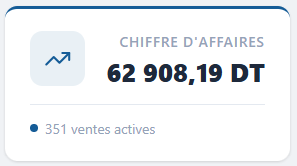
\includegraphics[width=0.6\textwidth]{images/tdb_ca_card.png}
  \caption{Indicateur KPI — Chiffre d'affaires total}
\end{figure}

Nous avons opté pour une \textbf{carte avec icône} pour afficher les indicateurs
synthétiques tels que le chiffre d'affaires total, le panier moyen et le taux de
croissance. Ce format permet une lecture immédiate des valeurs clés sans interprétation
visuelle supplémentaire.

\begin{figure}[H]
  \centering
  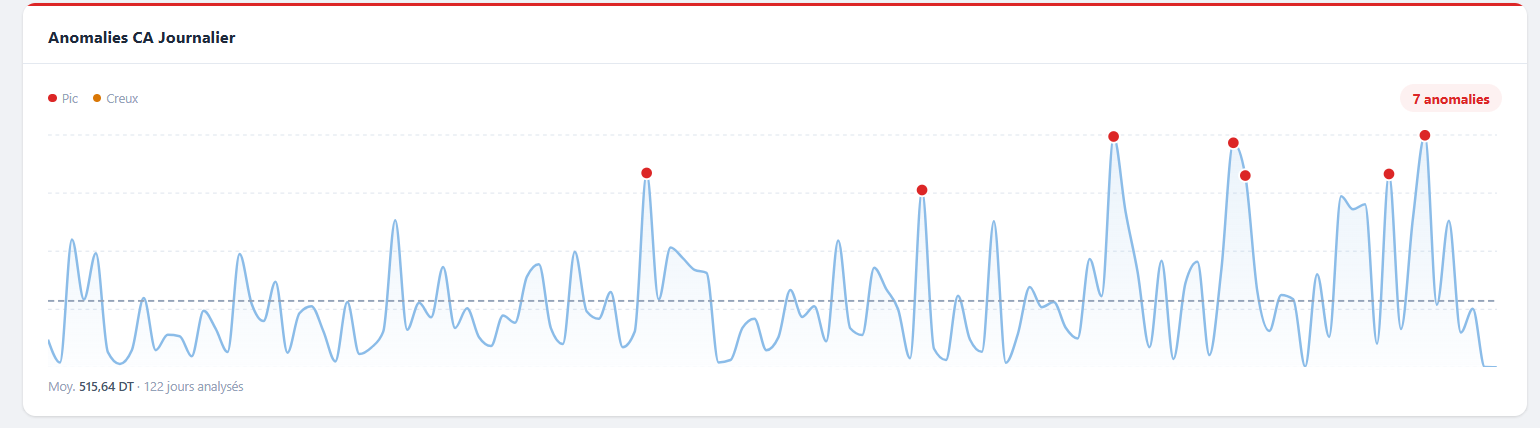
\includegraphics[width=\textwidth]{images/tdb_ca_anomalies.png}
  \caption{Anomalies CA Journalier — Graphique en courbe avec détection de pics}
\end{figure}

Nous avons choisi un \textbf{graphique en courbe} pour les anomalies du CA journalier,
car il permet de visualiser l'évolution continue des ventes et de mettre en évidence
les pics anormaux (en rouge) détectés par le Z-score, avec la moyenne affichée en
ligne pointillée comme référence.

\begin{figure}[H]
  \centering
  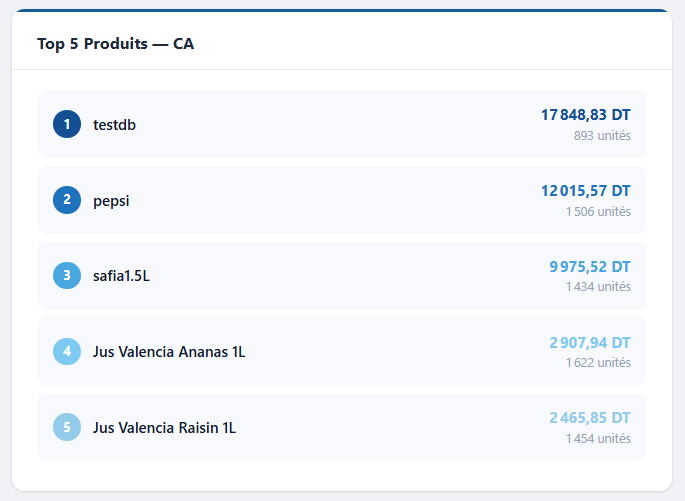
\includegraphics[width=0.65\textwidth]{images/tdb_ca_top5.png}
  \caption{Top 5 Produits par Chiffre d'affaires — Liste classée}
\end{figure}

Nous avons opté pour une \textbf{liste classée} pour le Top 5 des produits, car elle
offre une lecture directe du classement avec le CA et le nombre d'unités vendues pour
chaque produit, sans nécessiter d'interprétation graphique.

\begin{figure}[H]
  \centering
  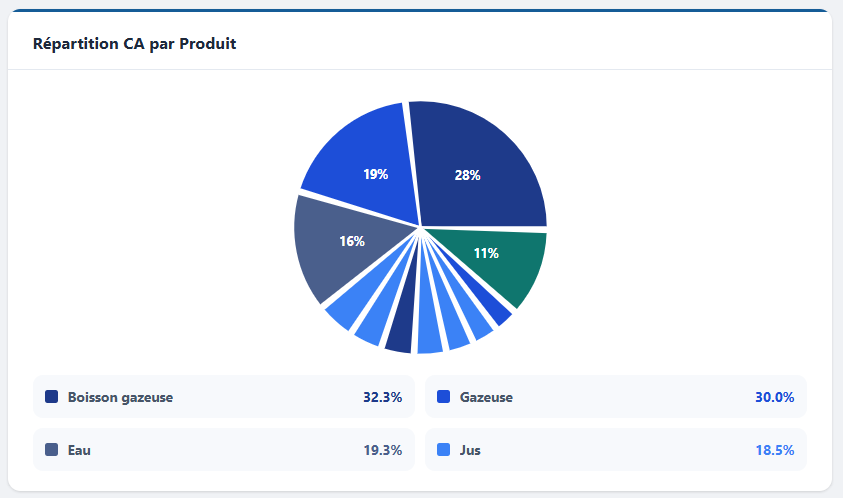
\includegraphics[width=0.65\textwidth]{images/tdb_ca_repartition_produit.png}
  \caption{Répartition du CA par Produit — Diagramme en secteurs}
\end{figure}

Nous avons sélectionné un \textbf{diagramme en secteurs} pour la répartition du CA
par produit et catégorie, car il illustre clairement la contribution proportionnelle
de chaque catégorie (Boisson gazeuse, Gazeuse, Eau, Jus) au chiffre d'affaires global.

%--- Tableau de bord Clients ---
\subsubsection*{Tableau de bord — Clients}

\begin{figure}[H]
  \centering
  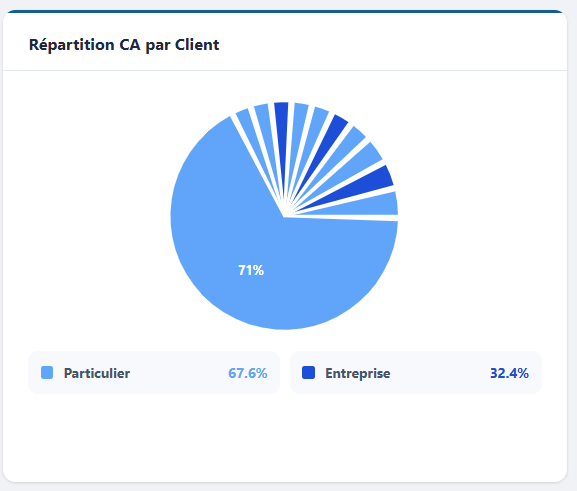
\includegraphics[width=0.65\textwidth]{images/tdb_clients_repartition.png}
  \caption{Répartition du CA par Client — Diagramme en secteurs}
\end{figure}

Nous avons opté pour un \textbf{diagramme en secteurs} pour la répartition du CA par
client et type (Particulier / Entreprise), car il représente efficacement la part de
chaque segment dans le chiffre d'affaires global et permet d'identifier rapidement
les types de clientèle les plus contributifs.

%--- Tableau de bord Facturation ---
\subsubsection*{Tableau de bord — Facturation}

\begin{figure}[H]
  \centering
  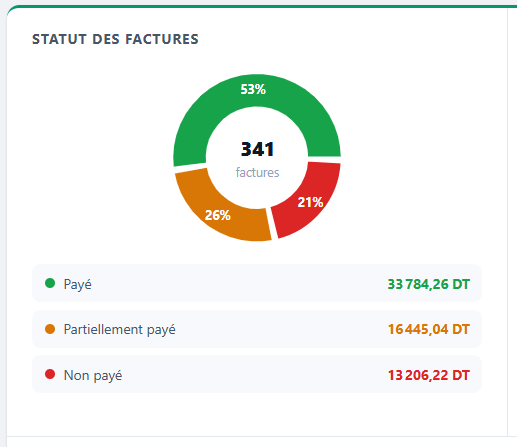
\includegraphics[width=0.55\textwidth]{images/tdb_fact_statut.png}
  \caption{Statut des Factures — Graphique en anneau (donut)}
\end{figure}

Nous avons sélectionné un \textbf{graphique en anneau (donut)} pour le statut des
factures, car il permet d'afficher simultanément le nombre total de factures au centre
(341 factures) et la répartition par statut — Payé (53\%), Partiellement payé (26\%),
Non payé (21\%) — en segments colorés immédiatement lisibles.

\begin{figure}[H]
  \centering
  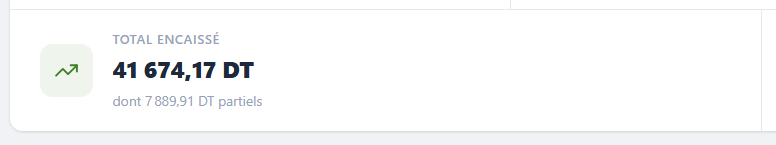
\includegraphics[width=0.65\textwidth]{images/tdb_fact_encaisse.png}
  \caption{Total Encaissé — Carte KPI}
\end{figure}

Nous avons opté pour une \textbf{carte KPI} pour les indicateurs financiers agrégés
tels que le total encaissé et le total attendu, car ce format met en valeur les
montants clés et leur détail (dont la part partielle) de manière synthétique et lisible.


\subsubsection*{Phase 3 : Mise en œuvre}

\textbf{Étape 9 --- Intégration et déploiement de la solution :}
Dans cette étape, nous avons déployé la solution complète au sein de
l'environnement de l'entreprise, en intégrant l'ensemble des modules développés
(voir Chapitre~5, page~\pageref{sec:ch5:impl}).

\newpage

%----------------------------------
\section{Module de Prévision et d'Analyse Intelligente}
%----------------------------------

\subsection{Fondements théoriques}

\subsubsection{L'apprentissage automatique}

L'apprentissage automatique (Machine Learning) est une branche de l'intelligence
artificielle (IA) qui se concentre sur le développement d'algorithmes informatiques
qui s'améliorent automatiquement grâce à l'expérience et à l'utilisation de données.
Il permet à un système d'apprendre à partir de données et de prendre des décisions
ou de faire des prédictions sans avoir été explicitement programmé pour le faire
\cite{datacamp_ml}.

Dans notre projet, il constitue le socle du module de prévision, permettant d'anticiper
le chiffre d'affaires, de segmenter les clients et de détecter les risques de non-paiement.
Les méthodes d'apprentissage se divisent en deux grandes catégories.

\subsubsection{Apprentissage supervisé}

L'apprentissage supervisé est une approche de machine learning qui se définit par
l'utilisation d'ensembles de données étiquetés. Ces jeux de données sont conçus pour
entraîner ou « superviser » les algorithmes afin qu'ils classifient les données ou
prédisent les résultats avec précision. Cette approche a été appliquée dans notre
projet pour prévoir le chiffre d'affaires et les ventes par produit \cite{ibm_supervised}.

\subsubsection{Apprentissage non supervisé}

L'apprentissage non supervisé utilise des algorithmes de machine learning pour analyser
et regrouper des ensembles de données non étiquetés. Ces algorithmes découvrent des
modèles cachés dans les données sans avoir besoin d'intervention humaine
\cite{ibm_supervised}.
Dans ce projet, cette approche permet de détecter les clients à risque et les mauvais
payeurs.

\subsubsection{Outils d'analyse intelligente}

Le tableau~\ref{tab:algorithmes} présente les principaux algorithmes mis en œuvre
dans notre module de prévision et d'analyse intelligente.

\vspace{6pt}

\begin{longtable}{|>{\bfseries\raggedright\arraybackslash}p{3.5cm}|>{\raggedright\arraybackslash}p{9cm}|}
\hline
\rowcolor{blue!20}
\textcolor{black}{\textbf{Algorithme}} &
\textcolor{black}{\textbf{Description}} \\
\hline
\endfirsthead
\hline
\rowcolor{blue!20}
\textcolor{black}{\textbf{Algorithme}} &
\textcolor{black}{\textbf{Description}} \\
\hline
\endhead
Régression Linéaire Simple &
La régression linéaire est une technique d'analyse de données qui prédit la valeur
de données inconnues en utilisant une autre valeur de données apparentée et connue.
Elle modélise mathématiquement la variable dépendante et la variable indépendante
sous forme d'équation linéaire \cite{aws_regression}. \\
\hline
K-Means &
Le clustering k-means est un algorithme d'apprentissage non supervisé utilisé dans
le partitionnement de données, qui regroupe les points de données non étiquetés
en groupes ou clusters \cite{ibm_kmeans}. \\
\hline
RFM &
La segmentation RFM est une approche de classification des clients basée sur la
Récence de leur dernier achat, la Fréquence des transactions et le Montant total
dépensé \cite{dinmo_rfm}. \\
\hline
Isolation Forest &
Isolation Forest est un algorithme de machine learning non supervisé qui identifie
les anomalies dans les données en les isolant via des partitionnements aléatoires
au sein d'un ensemble d'arbres de décision \cite{datacamp_iforest}. \\
\hline
\caption{Outils d'analyse intelligente}
\label{tab:algorithmes}
\end{longtable}

